\documentclass{chi2009}

\usepackage{url, graphicx, subfigure}
\usepackage{listings}

\hyphenation{ma-kum-ba}
\begin{document}

\title{Interactive Systems by Novice Programmers:\\ a %Declarative and 
Query-Centric Approach}

% TODO camera-ready: add reference to our own C&T work! 
\numberofauthors{2}
\author{
  \alignauthor Cristian Bogdan\\
    \affaddr{School of Computer Science and Communication}\\
    \affaddr{Royal Institute of Technology, Stockholm, Sweden}\\
    \email{cristi@csc.kth.se}
  \alignauthor Rudolf Mayer\\
    \affaddr{Institute of Software Technology and Interactive Systems}\\
    \affaddr{Vienna University of Technology, Austria}\\
    \email{mayer@ifs.tuwien.ac.at}
}

\maketitle
\begin{abstract}
Programing interactive systems is an expensive task. It has been long known that the part of the development cost of an application spent on the user interface accounts for 
%a large proportion (approx. 50\%) 
about half
of the total cost of the project 
%\cite{Myers92surveyon}. 
In this paper we introduce an approach to produce user interface based on queries, which made possible the development and maintenance of a large interactive applications by novice programmers over a long period, in 
% which we perceive to be
a sustainable interactive system development process. We claim that such productivity and sustainability with novice programmers is a good evidence for the power of the query-centric approach in user-interface programming. 
%Even if the current state of our declarative query-centric user interface generation technology 
%that we present, Makumba, 
%is focused on web applications, we will show how the query-centric approach can be used to generate other types of user interfaces, from Web 2.0 interfaces to more traditional GUIs.
\end{abstract}

\section{Introduction}\label{sec:intro}
Programming user interfaces is generally regarded as expensive and challenging.  It has been long known that the part of the development cost of an application spent on the user interface accounts for about half of the total cost of the project \cite{Myers92surveyon}. The state of the art in interactive system programming is often focused on separation of concerns, in architectural patterns such as Model-View-Controller (MVC). The user interface is engineered as one part of a modular system, often of equal or lower importance comparing to other modules. In effect, the preferred programming environments for developing user interfaces are dominated by the environments used in the rest of the system.

In this paper we describe the design and current developments of a framework (Makumba) that permits the realization of a system by mostly describing its interface, thereby driving the system development by the development of its user interface, and concentrating most of the system code in the user interface. While this brings compromises in regard to separation of concerns, it has been shown to be easy to learn even by novice programmers and to sustain the development of large systems (2000 code units) in large distributed teams (20 geographically distributed programmers) over a long period (over 8 years). We regard as the key to such positive measures is the description of user interfaces around queries, and combining the query language (an object-oriented variant of SQL) with a simple interface description language (HTML in this case). Even if currently the systems developed with our framework are Web systems and therefore support lower interactivity, we believe that the query-centric principle for describing interfaces can be applied elsewhere, and we are in the process of developing proofs of concept for this idea.

Model–View–Controller (MVC) \cite{reenskaug1979mvc1} is a pattern for software architectures. The pattern separates different concerns: the data representation, the domain or application logic, and the user interface. This allows each aspect to be developped independently from the others.
The model is the domain-specific representation of the data; there are no constraints upon the the data access layer below the model, which is understood to be encapsulated by the model. The view is responsible for rendering the model (and its data) for user interaction, generally by using interface widgets. For a  single model, multiple views can exist. The views can take many forms, such as a desktop application, a teller, or a web application.
The controller is receiving the input from the user, and processes it, which may result in changes in the data. Finally, the controller issues a response, which might be displayed by the view.

The MVC has been widely adopted in software engineering, and is also considered good practice for web applications. In these settings, the view is generally the HTML, while the controller receives input via HTML forms and subsequent GET/POST requests. The model is generally not different than in other, conventional applications. A range of web development frameworks support MVC in one form or another. One example in particular is Apache  Struts\footnote{http://struts.apache.org}, which provides the application developer with a tag library to create an interactive, form-based view, a response handler that is handling control, in combination with a request handler provided by the user, containing the application logic. No direct support is provided for the model, though.



%The Intranet of an European-wide organization had just over 600 dynamic pages at its launch in 2002. The Intranet grew steadily in both size and functionality and at the end of 2008 it has almost 2000 dynamic pages. Throughout, except for a few glitches, the system was highly available and fast. Today the Intranet has around 2000 users from among the organization members, and its public part can be accessed by 4000-5000 organization customers at a time.

%Such figures would not be surprising for a professional international organization, which hires or outsources professional programmers and system administrators, and can follow a well-defined development process based on established software and web-engineering concepts and techniques.
%The figures are however unusual for a voluntary student organization, whose IT crew (referred to as the Tech Committee) is made of amateur voluntary student programmers who often do not study Computer Science or related subjects, or are at the early stages of their education. 
%Since 2002, the Tech Committee had over 10 active members at any given time, and the Intranet was extended with more and more subsystems even if about one third of the Tech Committee membership was renewed each year. Reflection and analysis from a technology design perspective on this {\it sustainability}  is the subject matter of this paper. We assert that the design of the technology used to build the Intranet, called Makumba, is a determining factor in this sustainability. We also assert that since a technology worked well in a setting with so little development skill, its relevance for the web development community appears promising.



%We therefore designed a web application development framework which is relaxed in its constraints on formalization, but still enforces a certain development process by it's very own design, and results in web-application which are based on well-known software and web engineering concepts (such as aspect-oriented programming and MVC) by its very nature. Further, we put a specific emphasize on the code-base of the application to be in plain text rather than in visual models or bound to a specific CASE tool or IDE, and thus being allowed to be modified very easily from different operating systems with any kind of text-editing tool available. For the most basic beginners, we also developed a specific browser based tool that provides editing and revision control support, and can be accessed ubiquitously.

%Makumba is a framework for developing data-driven web applications, designed for students who do not necessarily know how to program initially. It covers the whole  web application spectrum, from creating the relational database tables and indexes, through creating, updating, and removing objects in the database, through calling back in Java application logic, to providing data presentation in HTML. On many of these fronts, Makumba is different from the state of the art, yet its designers have followed closely the evolutions along the years, using technology elements that were considered suitable, such as Java Server Pages and the Tomcat Servlet engine. Still, other technology elements that are usually chosen in the professional Java realm today, such as Struts,
%Hibernate, Spring, Enterprise Java Beans, Java Data Objects were partially or totally left out of the Makumba design. Web and data-driven application programming patterns like Data Access Object (DAO) and Data Transfer Object (DTO) are not adhered to, while patterns such as Model-View-Controller are partially adhered to and partially circumvented resulting in simpler code, lower code interdependence, better learning curve due to code simplicity, and intuitiveness. 

%Makumba also has a different programming language focus. 




%Among other popular web application frameworks related to the design of Makumba, but not based on the Java programming language, is for example Ruby on Rails (RoR)\footnote{http://rubyonrails.org/}. RoR is intended for the agile software development method, focused on rapid application development and short iteration cycles.

%In this paper we will  reflect on why our design ended up being different from the state of the art, yet still it was successful in this particular setting. We will first introduce the student organization, its group of web application (Intranet) programmers, and the applications they develop and maintain. A presentation of Makumba design follows, with the constraints that shaped it. We then present an evaluation of the technology done with the developers, focusing especially on learning. In the discussion we compare various aspects of Makumba design, learning and use with the corresponding aspects of widely used technologies and patterns for data-driven web development today. We also discuss how some widely used patterns and principles, like Data Access Object, are not used in Makumba applications, and consider the benefits of this "common practice amendment".

%\section{The setting for Makumba design and use}\label{sec:setting}
%The student organization running the Intranet of our interest was grounded in 1988 and is currently present in 80 mainly technical universities across 30 European countries, and has at the moment about 2,500 student members. The Intranet is supporting the activities of the organization, and consists of several integrated subsystems: an application system which registers student applications to the complementary education courses, an internal document archive and member profile management system, a "virtual jobfair" allowing companies to post job adverts, and students to post their profiles. Besides heavily extending and integrating the above sub-systems, several Intranet features were added (using Makumba) since its inception: a Wiki, email archives for the organization's over 500 mailing lists, a training database, a survey-engine, a career-newsletter, and a unique sign-in system that allowed students to share their accounts between various sub-systems, etc. Such new sub-systems, as well as adding more and advanced features to the existing ones, account for the growth of the Intranet code base.

%The Tech Committee is the team in charge of developing and maintaining the Intranet, as well as supporting it with activities such as helpdesk. The committee also coordinates activities of interaction design for further new areas of the Intranet. Administration of the Intranet, as well as of communication systems such as e-mail are also Tech Committee responsibilities. In its early (less sustainable) days, the Tech Committee consisted of 1-5 members who were mainly responsible for the individual systems and had difficulties backing each other up when they did not have time for voluntary commitment. Tech Committee membership levels increased after 2002 (constantly around 20), and new members are usually attracted in international meetings with a three-hour Makumba training, including exercises in making dynamic pages that browse Intranet data in various ways, improving existing Intranet pages, followed by assignment of more complex Intranet-related tasks.


% TODO more about the training, or after it: are they given Intranet tasks? Do they do Intranet-based exercises to change some interface or browse some Intranet data?
% rudi: in the training, they normally don't do Intranet related tasks, they do completely new pages. they start from a given MDD, and then do the full range: list, object, newForm, and then for the more advanced ones also editForm, deleteLink, mak:count() & co.
% TODO rudi: not clear here, do you just want to describe the recruiting, or also the first path in ITC

%It is important to emphasize that the Tech committee members are not formally trained, and are not paid. There are thus specific \textit{motivation} and \textit{learning} aspects in their activity. To be motivated to work without pay in a programming community, a Tech Committee member needs to be able to see very soon that they can contribute, i.e. that they can make a web application element (a JSP page) that displays Intranet data in some new way. Having passed this learning threshold (designed into Makumba to be low) that allows them to get involved, members have still some learning to do, and the essential aspect of such learning is that it is \textit {learning in doing}, without formal training, typically together with peers, or looking at what they have done. During such learning it is important that the members follow a smooth learning path, which, if possible should also be designed into technology \cite{bogdan_mayer09}.

%--------

%\subsection{Amateur software development}\label{sec:amateur_devel}

% i keep this because i think that something about the parallel with open source needs be made

%It is useful to characterize amateur software development such as hackers \cite{levy94} or open source \cite{kollock99} as amateur communities 
%because Tech Committee is a less professional (pre-professional) correspondent of such communities. 
%In such communities, code challenges are hardly exhaustible, as programming a machine leads to a rich set of contingencies, bringing along lots of 'trial and error'. 
%It is also easy to open new contingency spaces partly due to the immateriality of the working artifact, new projects, or project modules can always be started, or the existing ones can be re-organized ("refactored" in the professional jargon). For a newcomer, the complex architecture of large software projects adds to the challenge, and their skills of mastering the programming language will not be enough, they will also have to learn the way the project was organized.
%Code is shared typically via plain text messages, and carefully examined before being committed to the code repository, which suggests another amateur community feature, related to the notion of audience, the \textit{peer review} of challenge addressing. 
%Plain text is regarded as a very suitable medium for such distributed development and review efforts \cite{yamauchi00}. 
%Another important part of the community audience is its public, which can be an important motivation factor: for very generic projects it may be the world at large (e.g. in the case of an open source operating system kernel, an office suite), or very specialized professionals and amateurs in the software development field (e.g. for an open source compiler suite).

\section{Makumba design}\label{sec:makumba}

%Much industrial web development projects are written around procedural or object-oriented languages like  Java. While written in Java and its applications employing some Java code, Makumba programming code is mostly constituted by database queries, hence we call it a \textit{query-centric} technology. As we will show in this paper, we regard this ingredient as very important for the success of the Makumba-based Intranet and we are currently building up on this Makumba aspect.

We will illustrate the constraints that shaped the Makumba design during the development of a large Intranet within an international student organization.  Some of the constraints became apparent when they attempted to port previously existing applications to Lotus Notes and Domino, in a bid to reduce the number of technologies that the student developers have to master in order to maintain and develop the Intranet. % This aim was highly motivated given the high change of members actively developing, and the relative short time they stay in the student organization and the Tech Committee.
A framework was needed that can be used by a \textit{highly distributed team}. Most developers work alone, as they are not co-located with other developers. They meet face-to-face a few times a year, but most communication and coordination are carried out online. In this context, the Lotus Notes experience has quickly revealed that graphical modeling and programming techniques are difficult to work with in such a setting: questions that the novice members may have are hard to answer by other developers; communication needs to involve screen-shots or textual descriptions of graphical modeling elements. The use of plain text in other highly distributed programming settings, such as open source projects, is considered as an important factor contributing to the success of these communities \cite{yamauchi00}. 

Unlike in a professional development shop, or in an open-source programming setting, developers using Makumba have a wide variety of programming skill levels, some of them not having formal programming training at all. \textit{Accommodating novice programmers} was thus another important design constraint.
% Makumba needed to assume very little initial knowledge of the developers, sometimes limited to very basic HTML knowledge. 
A consequence of this has been the important focus on a natural-language inspired programming language, the Structured Query Language (SQL), which can be learned by new members by simply relying on their English. It is possible to build large parts of Makumba systems with only HTML and SQL knowledge. Makumba is thus a \textit{query-centric} framework in its design, i.e. most of its definitions, rules and instructions can be defined in queries. Thus, common to all levels is the usage of a query language, which can either be the Hibernate\footnote{http://www.hibernate.org/}  Query Language (HQL), or Makumba's own Query Language (MQL) which is a HQL subset. % Both query languages provide an object-oriented extension to the Structured Query Language, where MQL is explicitly simplifying the syntax for joins between different database tables.

Another consequence of the `novice programmer' constraint became visible when working with Lotus Notes, which provides developers with long lists of features, in which novice  voluntary developers easily got lost. \textit{Providing a small feature set} was thus another principle adopted, which resulted in e.g. a small number of data types offered to  Makumba developers. Besides providing a low entry point for novice programmers, it is known that novices often learn by looking at existing code, so it became important to ensure good \textit{code legibility} in a programming unit (JSP page) as well as \textit{easy code navigation} to facilitate finding scripts of interest in a large system as the Intranet.

In the context of the unexperienced developer group, it was not  to be expected that many in the developer team would have knowledge of architectural principles for large (web) applications. Therefore there was a need for the framework to ensure (or even enforce) a certain degree of \textit{separation of concerns} as recommended by the MVC pattern.
%  in the Aspect-oriented Programming (AOP) \cite{Kiczales97aspect-orientedprogramming} perspective. 
This is achieved by using  different files for data description, data presentation and data modification, and also by using different languages for the respective concerns. This has guided the developer team in maintaining a healthy architecture in the long run, and also served an educational purpose, by acquainting unexperienced developers with the separation of concerns principle. To address this design constraint, Makumba organizes a system in three major parts, the \textit{Makumba Data Definition}, the \textit{JSP level} and the \textit{business logic}, which we will introduce below. However, as we will illustrate, Makumba design makes a tradeoff in regard to MVC, which we will discuss later.

\subsection{Model data: Makumba Data Definitions}
The \textit{Makumba Data Definition} (MDD) describes data structures and relations between them. MDDs are simple lists of data fields, with name and type; the number of data types available is deliberately kept small and to a minimum, to reduce complexity. The most used data types comprise `primitive types' such as int, real, char, and dates, and `structural types' such as pointers and sets, which are references to other data types, and enumeration types. An example of an MDD can be seen in Listing \ref{list:mdd} for the data type `Student".

Additionally to defining the mere data structure, Makumba also allows to define validation rules the data has to comply to when created or modified. These rules can be specified in the form of `query fragments" (expressions in MQL or HQL), and are automatically and transparently composed to complete queries by Makumba. Writing data validation rules in the form of query fragments implies that a great deal of the controller-related tasks can be accomplished without the use of a procedural programming language.

\lstset{basicstyle=\small, captionpos=b, caption=Makumba Data Definition "Student", label=list:mdd, frame=shadowbox}
\begin{lstlisting}
name = char[50]
birthdate = date
hobbies = text

education = set
education->name = char[50]
education->university = ptr University
education->graduation = date
\end{lstlisting}

\subsection{View: JSP Level}
The \textit{JSP level} is primarily the user-interface level, and is technically a tag library for the Java Server Pages technology, allowing the display and changing of the data stored in a database and described in MDDs. The number of tags needed to perform the most basic operations is again kept very simple. An example of displaying data is given in Listing \ref{list:mak}, which shows the code required to display a list of students and, for each student, their completed studies; the data for this list is described in the aforementioned `Student" MDD (Listing \ref{list:mdd}).

\lstset{basicstyle=\small, captionpos=b, caption=Example of viewing data with the Makumba JSP tag library, label=list:mak, frame=shadowbox}
\begin{lstlisting}
<mak:list from="Student s">
 Name: <mak:value expr="s.name"/> <br/>
 Born on <mak:value expr="s.birthdate"/><br/>
 Completed studies:
 <mak:list from="s.education e"
      where="e.gradDate < now()">
  <mak:value expr="e.name"/>
  (<mak:value expr="e.university.name"/>),
 </mak:list>
 <br/>
</mak:list>
\end{lstlisting}

The example uses two tags: mak:list to specify the data definition to retrieve data from, and basic query constraints via the `where' attribute, and mak:value to indicate which fields to display. Notably, composing the query needed to retrieve the data from the database, i.e. the SQL joins and data projections are generated automatically and transparently from notations like ``s.education´´ and ``s.surname´´ respectively. Therefore working with a Makumba JSP would typically not require as much knowledge as using SQL by itself. Note that mak:lists can be nested into each other, and even in that case Makumba will generate exactly one query per mak:list. This optimization leads to a minimum number of queries sent to the database back-end, thereby honoring the single most important performance factor in data-driven web applications today.

Editing objects is done via forms, on a familiar note with HTML, thus helping the programmers in their learning.  Listing  \ref{form:mak} shows the mak:editForm and mak:input tags. The tags mak:newForm and mak:delete allow for the other typical operations. Rendering of the inputs into text fields, combo-boxes or date-choosers is done automatically, based on the type information provided in the MDD. To edit chains of related objects, forms can be embedded in other forms, as shown in Listing \ref{form:mak}.

\lstset{basicstyle=\small, captionpos=b, caption=Example of changing data with the Makumba JSP tag library, label=form:mak, frame=shadowbox}
\begin{lstlisting}
<mak:object from="Student s" where="s=:student">
<mak:editForm object="s" action="somePage" >
 Name: <mak:input field="s.name"/> <br/>
 Born on: <mak:input field="s.birthdate"/><br/>
 Edit  studies:
 <mak:list from="s.education e"> 
  <mak:editForm object="e">
   name <mak:input field="e.name"/> <br>      
   graduation <mak:input field="e.graduation"/>
   university <mak:input field="e.university"/>
   </mak:editForm>
 <mak:list>
 <input type="submit">
<mak:editForm>
</mak:object>
\end{lstlisting}

Makumba supports model-driven development methods, as it can automatically create forms and lists by merely specifying the data definition to be used in the form or list, and generating pages by taking information on the data fields from the Makumba Data Definitions.%; programming-wise, this can be triggered by not specifying the mak:values or mak:inputs in the mak:list and mak:form. 
Thus, data definition changes are instantly and seamlessly propagated to the JSP level, which makes it ideally suited for Rapid Application Development and fast prototyping. %A weaker form of model-driven development support, which allows more influence on the layout of the created page, comes with tools creating the needed JSP pages from the data definitions, applying user-specifiable templates.

Unlike a few other technologies proposed today (e.g Struts), Makumba does not employ a navigation model. Instead, the HTML links and form actions are used to determine the next page to execute, thereby building upon its programmers' familiarity with HTML. Extra code to execute for authentication, authorization, validation, and further business rules (described below) is determined automatically according to the data type (MDD) used. This results in a quite scalable design, letting developers create independent pages, while still centralizing the business rules. % It is interesting to note that it was at several points considered to 'outsource` some of the Makumba code and features by integrating the Struts technology. It was however deemed that the Struts centralization of action configuration in one single XML file can break the low interdependency between developers that Makumba achieves today, thereby affecting team scalability. It would also have added to the configuration work needed to set up a Makumba application, which is kept to a minimum by design.

To support more interactivity we have recently added support for `page sections´ which can be refreshed, hidden or shown when a certain `event´ occurs. The event can be a JavaScript event of a user interface element in the generated HTML, a timer event or a change event propagated from the server. This feature also serves ``proof of concept´´ showing that the query-centric approach to user interface description can also be employed for systems that employ more interactive elements than page navigation and form submission (Web 1.0).

\subsection{Model constraints: Business Logics}
The \textit{business logic} (BL) describes, in the Java programming language, ``business rules´´ that restrict the changing of data, and provide authentication and authorization mechanisms. Makumba provides a Java API towards the data base, thus business logics classes can also be utilized to perform processing of complex queries that are harder to generate via the Makumba JSP level. Thus, the simplicity of use of the JSP level does not impose any limit on application functionality. To provide business logic that will be called before e.g. a Student creation, the programmer has to provide a Java method named \textit{on\_newStudent()} which will receive as parameters handlers to the page parameters, the session and the database.

%Initially Makumba was designed and developer under another, more neutral name ("Metadata"). When a more specific name was sought, designers remembered of a name that was well-known to many student organization members: the Makumba party. The name was known but not the actual meaning because members who had attended a Makumba party usually described as like below, without further detail. 
%\begin{quotation}
%	"You enter a room, the lights are turned off and then somebody tells the Makumba joke."
%\end{quotation}

%Ironically, the main Makumba designer had never attended a Makumba party, but knowing about its existence and its fame within the organization was enough to decide on the name.


Having a complex language like Java to express business logic was however regarded as a shortcoming in relation to the simpler programming languages used at the JSP level. Thus, in the current Makumba design iteration, to capitalize on the apparent easiness with which the developers approached query fragments at the JSP level, we decided to attempt to describe as much as possible of business logics using query fragments, directly in MDDs, thereby concentrating the entire Model MVC concern in the MDDs and facilitating developers' navigation through code. One example is the introduction of \textit{data integrity constraints} in the MDD layer, which are expressed as query fragments. 

A more complex example of reducing the need for Java code is the \textit{implicit data access layer} that analyzes the queries which require data in the JSPs (through tags such as mak:list) and apply MDD-defined query language functions that are appended (through in-lining)  to the generated queries to determine whether the  logged-in user has access to the respective data. This will replace a lot of Business Logics code that is currently doing the same job at the Java level. Listing \ref{qfauth:mak} shows an example that, once added to the Student MDD in Listing \ref{list:mdd}. would make the Student object only readable by their owner, or by administrator students. The current Java BL code achieving the same is much more verbose, due to the need of managing a transaction, retrieving an object, preparing a query and its parameters, retrieving its result set, etc.
\lstset{basicstyle=\small, captionpos=b, caption= query fragment authorization rule, label=qfauth:mak, frame=shadowbox}
\begin{lstlisting}
canRead() {actor(Student)=this 
                 OR actor(Student).admin=1 }
\end{lstlisting}
This query fragment will then be added transparently to all mak:lists attempting to fetch Student data. In such mak:lists, the programmer can define the default behavior of the containing page, which can be either to filter results which a user is not authorized to view, most suitable for a listing of several data records such as a list of all students, or showing an error message, which is especially useful when showing only one specific account, e.g. a specific member profile.



\subsection{A large Makumba system: the Intranet}
Table~\ref{tab:intranet-size} shows the evolution of the size of The Intranet since its launch seven years ago, detailed for the different technological levels MDD, JSP and BL. Additionally, the total number of code files is shown, along with the total lines of code (LOC). This data indicates quantitatively the project size afforded by Makumba, and the kind of `healthy' project growth that we argue Makumba can facilitate. The data also illustrates typical proportions of code types in a Makumba project: most code is in JSP scripts made predominantly of HTML and SQL-like code snippets, and there are 6-8 times fewer Java BL (business logic) files, and data definition (MDD) files are less than half the number of BLs, and are growing slower in number than JSPs and BLs. There was a rather high amount of MDD files defined in the beginning of the Intranet, representing data types used already in the ancestor systems. Even though more data definitions have been added over time, a certain saturation level with only minor additions was reached in the last years. It is not unexpected that the data definitions of an organization (its "domain model") change seldom after an initial development time. 

\begin{table}[t]
	\centering
	% TODO: explain LOC, etc? explain that all data is measured at the beginning of the year?
	% TODO: explain the drop from 2008 to 2009 needed? (due to removal of old BCC & public website pages in 2008, new ones have been added since late 2007, thus there were some `duplicates')
	\begin{tabular}{c|r|r|r|r|r|r}
		\hline
		\hline
		Year	& MDD	& JSP	& BL	& \# files	& LOC		& CVS	 \\
		\hline
		\hline
		2002 	& 42	& 676	& 80	& 801		& 78479 	& N/A	 \\ 
		\hline
		2003 	& 52	& 961	& 116	& 1132		& 104805 	& 1143	 \\ 
		\hline
		2004 	& 64	& 1208	& 140	& 1415		& 127873 	& 702	 \\ 
		\hline
		2005 	& 76	& 1354	& 190	& 1628		& 151801 	& 1324	 \\ 
		\hline
		2006 	& 99	& 1719	& 229	& 2062		& 175315 	& 1632	 \\ 
		\hline
		2007 	& 111	& 2135	& 287	& 2559		& 219456 	& 2391	 \\ 
		\hline
		2008 	& 114	& 1860	& 289	& 2304		& 196867 	& 1898	 \\ 
		\hline
		
% old data, # files & LOC from CVS-stat
% 		Year		& \# files 		& LOC		& MDDs	& JSPs	& BL \\
% 		\hline
% 		\hline
% 		2003		& 850			& 55,000	& 42	& 729	& 80\\
% 		\hline
% 		2004		& 1,200			& 75,000	& 52	& 1097	& 116\\
% 		\hline
% 		2005		& 1,700			& 85,000	& 64	& 1388	& 140\\
% 		\hline
% 		2006		& 2,300			& 132,000	& 76	& 1564	& 190\\
% 		\hline
% 		2007		& 3,050			& 200,000	& 99	& 2057	& 229\\
% 		\hline
% 		2008		& 3,550			& 305,000	& 111	& 2526	& 287\\
% 		\hline
% 		2009		& 3,750			& 312,000	& 114	& 2303	& 289\\
		\hline
		\hline
	\end{tabular}
	\caption{Size of the Intranet}
	\label{tab:intranet-size}
\end{table} 

\section{Evaluation of Makumba learning}\label{sec:techCommittee}
Throughout the Makumba design, the assumption was that it will be easy for students to read MDDs, and based on that, it will be possible for them to combine HTML and a subset of SQL (itself based on natural language) which they might know prior to start working with Makumba or might learn ``on the job´´. Later on, they would become interested in writing new business rules, and might learn procedural Java for that, maybe using previous knowledge of another procedural programming language. % This then would be the "learning path" assumed for a Makumba practitioner.

%In 2002 the first author evaluated the design of Makumba with a questionnaire that had 12 respondents. In 2005 the first author also ran a questionnaire with 32 respondents to asses the status of Tech Committee work and technology use, and thus indirectly look at its sustainability. Finally, both authors
We designed a questionnaire where 30 out of the 45 past (since 2003) and present members who were approached reflected on their activity in the Tech Committee over their whole 1-4 year-long membership period. %Questionnaire results are described in detail in \cite{bogdan_mayer09}, while here we will refer mostly to the questionnaire data on self-assessed learning.
Among the 30 survey respondents, the 
time of Tech Committee membership ranges from their activity starting around 2001, to fresh members that just joined in the second half of 2008. Also the educational background is diverse -- 13 members study computer science, computer engineering or informatics; the other respondents follow various other curricula, ranging from mechanical engineering to physics and biomedical engineering.  %Also, the membership duration in the committee varies, from 6 members that were active for around four years, to members that were (or currently are) active for one to two years. Most members had no knowledge of Makumba before joining.

% parade 2005: http://private.best.eu.org/survey/admin/listAnswers.jsp?survey=fn29yq1
% makumba 2008: http://private.best.eu.org/survey/admin/listAnswers.jsp?survey=cwu9pab



% number of files per type
% *** Viewing (list, object): 
% mak:list: 1097
% mak:object: 1102
% total unique viewing files: 1584 (~64%)
%
% *** Adding/Changing: 
% mak:newForm: 179
% mak:addForm: 79
% mak:editForm: 284
% mak:form: 167
% total unique form files: 596 (~24%)
%
% *** BL: 287 (~12%)

% TODO: describe why `active' column might have smaller numbers than others..
%Table~\ref{tab:itd-members} illustrates the number of active members in the Tech Committee since 2003, differentiated on the different levels of Makumba, and on their activity in newcomer (`peripheral') and old-timer (`core') members. This data was  extracted on the one hand from the latest questionnaire filled in by the members, and then refined and amended by some of the committee coordinators (for the year 2003, only the total number of active core and peripheral members could be estimated). It is interesting to note that while the overall number of active members increased over the years and stabilized in the last years, the (relative) number of members working on data definitions (MDD) was rather decreasing; this might be explained with the arrival at data maturity level as described above, and thus less work and challenges to take for the Tech Committee members, while plenty of challenge is left at other levels. An important sign of sustainability as we characterized it earlier is the sufficient number of members at both novice (peripheral) and expert (core) members active at all the Makumba usage levels at all times. The "learning paths" are thus well populated with community members.



%\subsection{Survey}\label{sec:techCommittee-survey}

%To attempt an understanding of the learning aspect of Makumba in the context of the Tech Committee, the participants were asked several questions on their self-assessed skill level on database design, SQL, general programming, Java, and three aspects of Makumba: JSP pages to view data, JSP pages to change (create, edit, and delete) data, and business logics (BL). The questions were asked repeatedly for several different points in time, namely when joining the committee, and after the first, second, third and fourth year of membership, and allowed answers from `no skills' via `little knowledge', `some experience' and `experienced' to `master'. To balance the self-assessments and to facilitate recall, the participants were further asked to estimate their contribution to the committee in that year, and to list the projects and technologies that they worked with in that year. Also to improve the quality of the self assessment, members were informed that the committee coordinators from their time of activity will review their answers.


%\begin{table}[t]
%	\centering
%	\begin{tabular}{c|r|r|r|r|r|r|r|r|}
%		\hline
%		\hline
%		Year 		& \multicolumn{2}{c|}{MDD} & \multicolumn{2}{c|}{JSP}	& \multicolumn{2}{c|}{BL}	& \multicolumn{2}{c|}{Active}	\\
%					& Per & Core				& Per & Core				& Per & Core				& Per & Core	\\
%		\hline
%		\hline
%		2003 &   &   &   &   &   &   & 4 & 5 \\
%		\hline
%		2004 & 3 & 4 & 7 & 3 & 3 & 3 & 6 & 5 \\
%		\hline
%		2005 & 5 & 6 & 8 & 11 & 7 & 3 & 8 & 13 \\
%		\hline
%		2006 & 7 & 8 & 9 & 12 & 9 & 3 & 10 & 12 \\
%		\hline
%		2007 & 7 & 7 & 14 & 9 & 10 & 5 & 12 & 11 \\
%		\hline
%		2008 & 6 & 5 & 13 & 7 & 6 & 7 & 12 & 8 \\
%		\hline
%		\hline
%% Summer meetings
%% 2003: http://private.best.eu.org/events/event.jsp?event=21-C-CJ-COM
%% 2004: http://private.best.eu.org/events/event.jsp?event=22-C-RI-COM
%% 2005: http://private.best.eu.org/events/event.jsp?event=23-C-LD-COM
%% 2006: http://private.best.eu.org/events/event.jsp?event=24-C-SF-COM
%% 2007: http://private.best.eu.org/events/event.jsp?event=25-C-TM-COM
%% 2008: http://private.best.eu.org/events/event.jsp?event=26-C-BE-COM
%	\end{tabular}
%	\caption{Members in the Tech Committee}
%	\label{tab:itd-members}
%\end{table} 

\begin{figure}[t]
  \label{fig:learning-technologies}
  \centering
  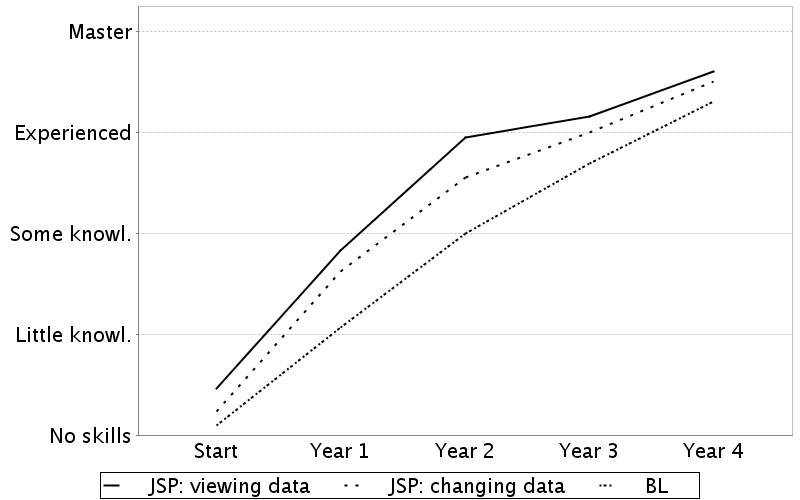
\includegraphics[width=0.7\columnwidth]{figures/learning-technologies}
  \caption{Learning curve for different aspects of Makumba}
\end{figure} 

Figure \ref{fig:learning-technologies} shows the averaged skill levels of all the members at different points in time, separated for three Makumba usage aspects: JSP for viewing data, JSP for modifying data, and BL. The data suggests that learning to view and display data at the JSP level is faster than handling forms to create, edit, and delete data. 
Since 64 \% of the Intranet files are viewing data, even medium level of Makumba JSP knowledge will give `access' to approximately two thirds of the Intranet programming units. 
Learning how to change data has a smaller impact, only 24\% of Intranet files are JSPs containing forms. 
Business Logics are the most difficult concept, especially in the first two years of membership, yet they only cover 12\% of the Intranet code. While this Java code is crucial for the Intranet functionality, the novice members have a lot of space to express and make themselves useful elsewhere. The BL code is expected to decrease dramatically when most Intranet business rules will be ported to query fragments of the kind shown in Listing \ref{qfauth:mak}.
Most members that stay in the committee for a longer period, however, master all levels of Makumba almost equally well. Such members can (and many do) continue working on the internals of Makumba itself  as a next step. While MDD editing skills are less and less actual, we can consider that currently the learning path milestones in the Tech Committee are: JSP viewing data, JSP changing data and BL.
%  To further illustrate the member skill evolutions, we have selected the charts of four individual members in Figure \ref{fig:learning-members}. This also shows that, although the dynamics vary a lot, the JSP data-changing skills almost always lag behind the JSP data view skills, and BL skill is acquired last. 

Overall, the per-year self-assessment results suggest that the learning path designed into Makumba has achieved its goal, allowing for members to have an easy start by visualizing data in JSP (which also requires MDD understanding), then starting to change data through JSP forms, and finally learning how to write business rules in Java.



%Two open questions concluded the questionnaire. The first one aimed at helping to assess how the members experience learning technologies in the Tech Committee. Several respondents emphasized the \textit{simplicity} and conciseness of Makumba code, therefore easiness to start working with, in various ways: as an intuitive link between code and result,  or as a praise to simplicity perceived as being able to express things in only one way, with a direct reference to people coming into and leaving the Tech Committee,  or as a technology that provides for rapid achievement, thereby encouraging further involvement. It is important for the Tech Committee in the international meetings to 'catch' people fast, by allowing them to realize that they can do something, that they can contribute. If this would not happen fast, the prospective new member might lose interest and maybe try to join another international team where contribution is more facile. A respondent emphasizes that "there is life" beyond the first simple steps, i.e. there are more complex things to be done, and Makumba accommodates for these as well. Several respondents compare Makumba with other Web development frameworks in this regard. More than one respondent referred explicitly to "non-IT people", thereby emphasizing the suitability for amateur settings.

%
%Respondents refer to their learning primarily from other members, sometimes even without explicit training and without even mastering the basics of the entry-level skill (HTML and SQL). Also learning by reading a mailing list is mentioned. Other informants report having asked questions on the Tech Committee mailing list and getting a multitude of good answers, also usable in the professional life of the then-amateur.
%Learning by reading examples (existing code) is emphasized by most respondents. Knowing how the Intranet is organized helps to find relevant code. A problem with learning Makumba is raised: since it is little known outside the student organization, there is no chance that some joining members already come in the Tech Committee with the skill.

%
%The last question asked the respondents for a comparison of Makumba with other technologies and frameworks aimed for web development. Many of the former or present members of the Tech Committee, currently working in IT jobs, were able to provide comparisons from a qualified professional perspective, with references to related technologies. Notably a number of members make architectural remarks, referring to some technical imperfections of Makumba, which does not provide a good separation between data model, its visualizations and the data change mechanisms (controllers). However most respondents regard this as an asset in the end, leading to easier programmer access to the data and higher maintainability.

\section{Discussion}\label{sec:disco}
The JSP level, where the user interfaces are described, is clearly the core of Makumba developer activity, with almost 90\% of the source files of a large, real-life system. This is also where the query-centric character of Makumba is most visible, by combining query fragments through mak:list, mak:value and mak:input tags. This Makumba View (in a MVC perspective) level is thus crucial to the framework's success, as most developers start at this level, and find it easy to get involved with viewing data, and then they move into writing pages that change data. 

%As emphasized in our design rationale, and apparently confirmed by our evaluation data, \textit{skill modularity} is a feature that led to the Makumba success in the Intranet project. The first such `module' has a low learning threshold (HTML and simplified SQL-queries), and the next modules provide developers with new challenge levels (e.g. Business Logic, with the procedural Java skill to be learned).

Especially for the entry-level modules (JSP), \textit{code legibility} is an important Makumba design feature, in such a context of learning in doing, from peers, or from the artifacts they produced. 
A major part of the Makumba JSP level simplicity and legibility is inherited from the corresponding feature of SQL queries, as legibility and intuitiveness were among its design principles, since it is based on natural language. Members who do not know SQL simply have to rely on their English to find their way around initially. This is further helped by Makumba JSP using a simplified form of SQL queries. Queries and query fragments are currently being introduced in the MDDs, with the aim of reducing the Java BL code, thus further emphasizing the Makumba \textit{query centric} character. Using plain text code rather than visual programming further helps the sharing and understanding of existing examples \cite{yamauchi00}. While we believe that model driven development is an important and productive movement, our experience runs contrary to many tendencies such as in WebML \cite{Ceri00webmodeling} to use graphical, rather than textual models.

Reflection on Makumba applications architecture leads us to two apparently contradictory considerations. On the one hand, Makumba imposes a widely accepted MVC rule, preventing developers from mixing business rules with data views. Many technologies in use by web developers (like PHP) do not enforce this separation, leading to lack of \textit{code scalability} of application development: application development can be started up fast, like with Makumba, but once applications grow large, problems start to occur due to not enforcing this major principle, affecting in the end sustainability. % Of course, trained and experienced programmers can avoid such problems also when using PHP, but this is more unlikely for novice, amateur developers as in our setting.

On the other hand, another principle, the separation of data view from data access (part of the MVC Model) is violated by Makumba in the design of its JSP level, since the queries that fetch the data necessary for presentation are part of the presentation units (JSP pages). %This issue was emphasized in questionnaire responses by several former developers, currently working with professional IT development. 
In mixing the data view and the data access, Makumba design ignores the Data Access Object and Data Transfer Object patterns usually employed in the industry, and make Makumba different from other agile development technologies like Ruby on Rails. This however has important code legibility consequences, as programmers only need to work with one file to understand how a unit of the JSP presentation layer works. Also the very code composition phase is eased a lot, allowing the students to contribute fast to the Intranet, which is very important for motivation. 

The mix of data access and data presentation also leads to \textit{easy code navigation}.  Makumba has fewer kinds of code files than other web application technologies, therefore requiring less navigation between files when performing a task. This helps the novices to make easier progress, and achieve better orientation when contributing to a large project like the Intranet. Furthermore, this source file compactness, especially at the JSP level, leads to little interdependency between the JSP source files. This allowed the Intranet to grow large in a number of independent directions without much dependency between its JSP units. While the multitude of JSP files still depend on the MDD and BL files, these are almost two orders of magnitude fewer in number, thus reducing the probability for conflict. This \textit{code scalability}  helps when several developers work on different parts of the Intranet, as they are not prone to affect each other's work, and thus the likely mistakes that a novice makes will not affect his or her peers. Such \textit{team scalability} at the JSP level is ideal for the sustainability of large web systems development.

As shown by this experience, Makumba allows the building of large Intranets by operating with only the presentation language (HTML for now, but other presentation forms are considered) and a query language. System performance and reliability are high, due to the Makumba query optimization, rivaling professional systems such as Enterprise Java Beans J2EE systems,  which are built in much more structured manners, in more complex programming languages like Java.  Besides JSP, such systems also employ Java for describing beans, sessions, data access and data transfer objects, and all these are interconnected with a multitude of XML files that lead to interdependencies with many parts of the system, thus reducing code scalability. While such complexity would clearly be beyond the reach of the novice programmers in our case, the Intranet they built can rival in complexity with many professional J2EE Intranets. This and previous observations question the need for a strict separation of concerns as enforced by J2EE to a large extent and other frameworks like RoR to a lesser extent.


\section{Related Work}\label{sec:related}
With the steady rise in importance of web-based applications, the processes and tools available for such web-based applications development has been studied intensively. A number of models for the (web-) development process has been proposed, trying to formalize the process with the goal of improving the quality of such web applications. Earlier models include the \textit{Object-Oriented Hypermedia Design Model} (OOHDM) \cite{schwabe1998ooa}, which introduces five different activities in the development process (requirements gathering, conceptual design, navigational design, abstract interface design and implementation), each of which is supported by a set of formalisms and methods, and yields a specific product. The \textit{Web Modeling Language} (WebML) \cite{Ceri00webmodeling} provides a visual notation for web-application design. It defines several different models as different steps in the process, mainly the structural model defining the data, the composition model specifying the content units, and the navigation model establishing the connection between those units. Tool-support for the development process is provided for example with WebRatio \cite{acerbis2004wit}. 
As well as Makumba, WebML allows the user to specify certain queries in the form of the Object Query Language OQL, which significantly simplifies multi-table queries as compared to SQL. Further, WebML allows to define so-called \textit{derived} attributes, which are basically fragments of OQL queries, similar to Makumba MDD-functions.

While especially WebML might well suit professional settings, the situation is different for voluntary novice programmers, especially in distributed development settings. As the amount and timing of work done depends entirely on the motivation and availability of the individual members of the organization, it is unfeasible in many ways to enforce a strict set of processes and work-flows to follow and specific tools to use. Applying too strict formalisms might in fact be counter-productive, as it might be perceived as a demotivating restriction on the development work. Also, installation effort required to start contributing should be kept to a minimum, especially when the contributor often change their working platform, using their home computer, university equipment, or other systems available while traveling.

%Hibernate\footnote{http://www.hibernate.org/} is a object persistence framework, and provides an alternative to the complex Enterprise Java Beans (EJB) framework, which is a part of the J2EE specification. Hibernate is built on idiomatic, transparent persistence of Java objects, and allows to express queries in its own Hibernate\footnote{http://www.hibernate.org/} Query Language (HQL), an extension of SQL. Makumba can work towards Hibernate-managed databases but it can also work without Hibernate (as it does in its largest application, the Intranet), using a subset of HQL.

%The technological base of Makumba is J2EE\footnote{http://java.sun.com/javaee/}, which is a well-known framework for enterprise and web application development, building on the Java programming language. While J2EE provides certain assistance for different aspects such as for example data object access and persistence, the complexity of the framework, and its partly lower-level application programmer interface (API) have called for a magnitude of web-application development frameworks building on top of J2EE. An overview of certain shortcomings of J2EE, and how they have been addresses by these frameworks, is given in \cite{johnson2005jdf}. Among those, Struts\footnote{http://struts.apache.org} adds support for separating the application in separate concerns using the Model-View-Controller (MVC) architecture, and provides support for building web-based forms. 


\section{Conclusions}\label{sec:conclusions}
Based on the Makumba experience we believe that query-centric technologies can gain a firm place among interactive system development frameworks today. Focus on  user interface description in a query-centric manner, can lead to good  code legibility, little code interdependence, easy code navigation,  helping the scalability of the code and the team maintaining it.  We also showed that mixing data access and data view can lead to important positive results although it is against general MVC concepts. We are currently working on data access determined in an implicit, declarative, and also query-centric way. 

%ACKNOWLEDGMENTS are optional
\section{Acknowledgments}\label{sec:acknowledgments}
Thanks to the students who worked hard to overcome Makumba imperfections during its  and to make the Intranet what it is today, while also taking time to answer our surveys.  Thanks are also due to all the Makumba contributors. 


\bibliographystyle{abbrv}
\bibliography{eics2010-makumba}

\end{document}
